\section{Transformer}
Τα αναδρομικά νευρωνικά δίκτυα αλλά και τα \emph{LSTM} μονοπωλούσαν για αρκετά χρόνια την επίλυση προβλημάτων που απαιτούσαν επεξεργασία σειριακής πληροφορίας, όπως αυτά των \emph{NLP} και \emph{NLU}. Τα \emph{Transformer} παρουσιάστηκαν για πρώτη φορά το $2017$ στο άρθρο \emph{"Attention is all you need"} \cite{attention} και έφεραν στο προσκήνιο μία νέα αρχιτεκτονική για την επίλυση τέτοιου είδους προβλημάτων, \autoref{fig:transformer}. Πιο συγκεκριμένα, το \emph{Transformer} αποτελείται από $N$ επίπεδα κωδικοποίησης, $N$ επίπεδα αποκωδικοποίησης και εστιάζει στη μέθοδο της προσοχής (\emph{attention}) για να διακρίνει ποια κομμάτια της εισόδου είναι πιο σημαντικά.

\begin{figure}[!ht]
  \centering
  \captionsetup{justification=centering}
  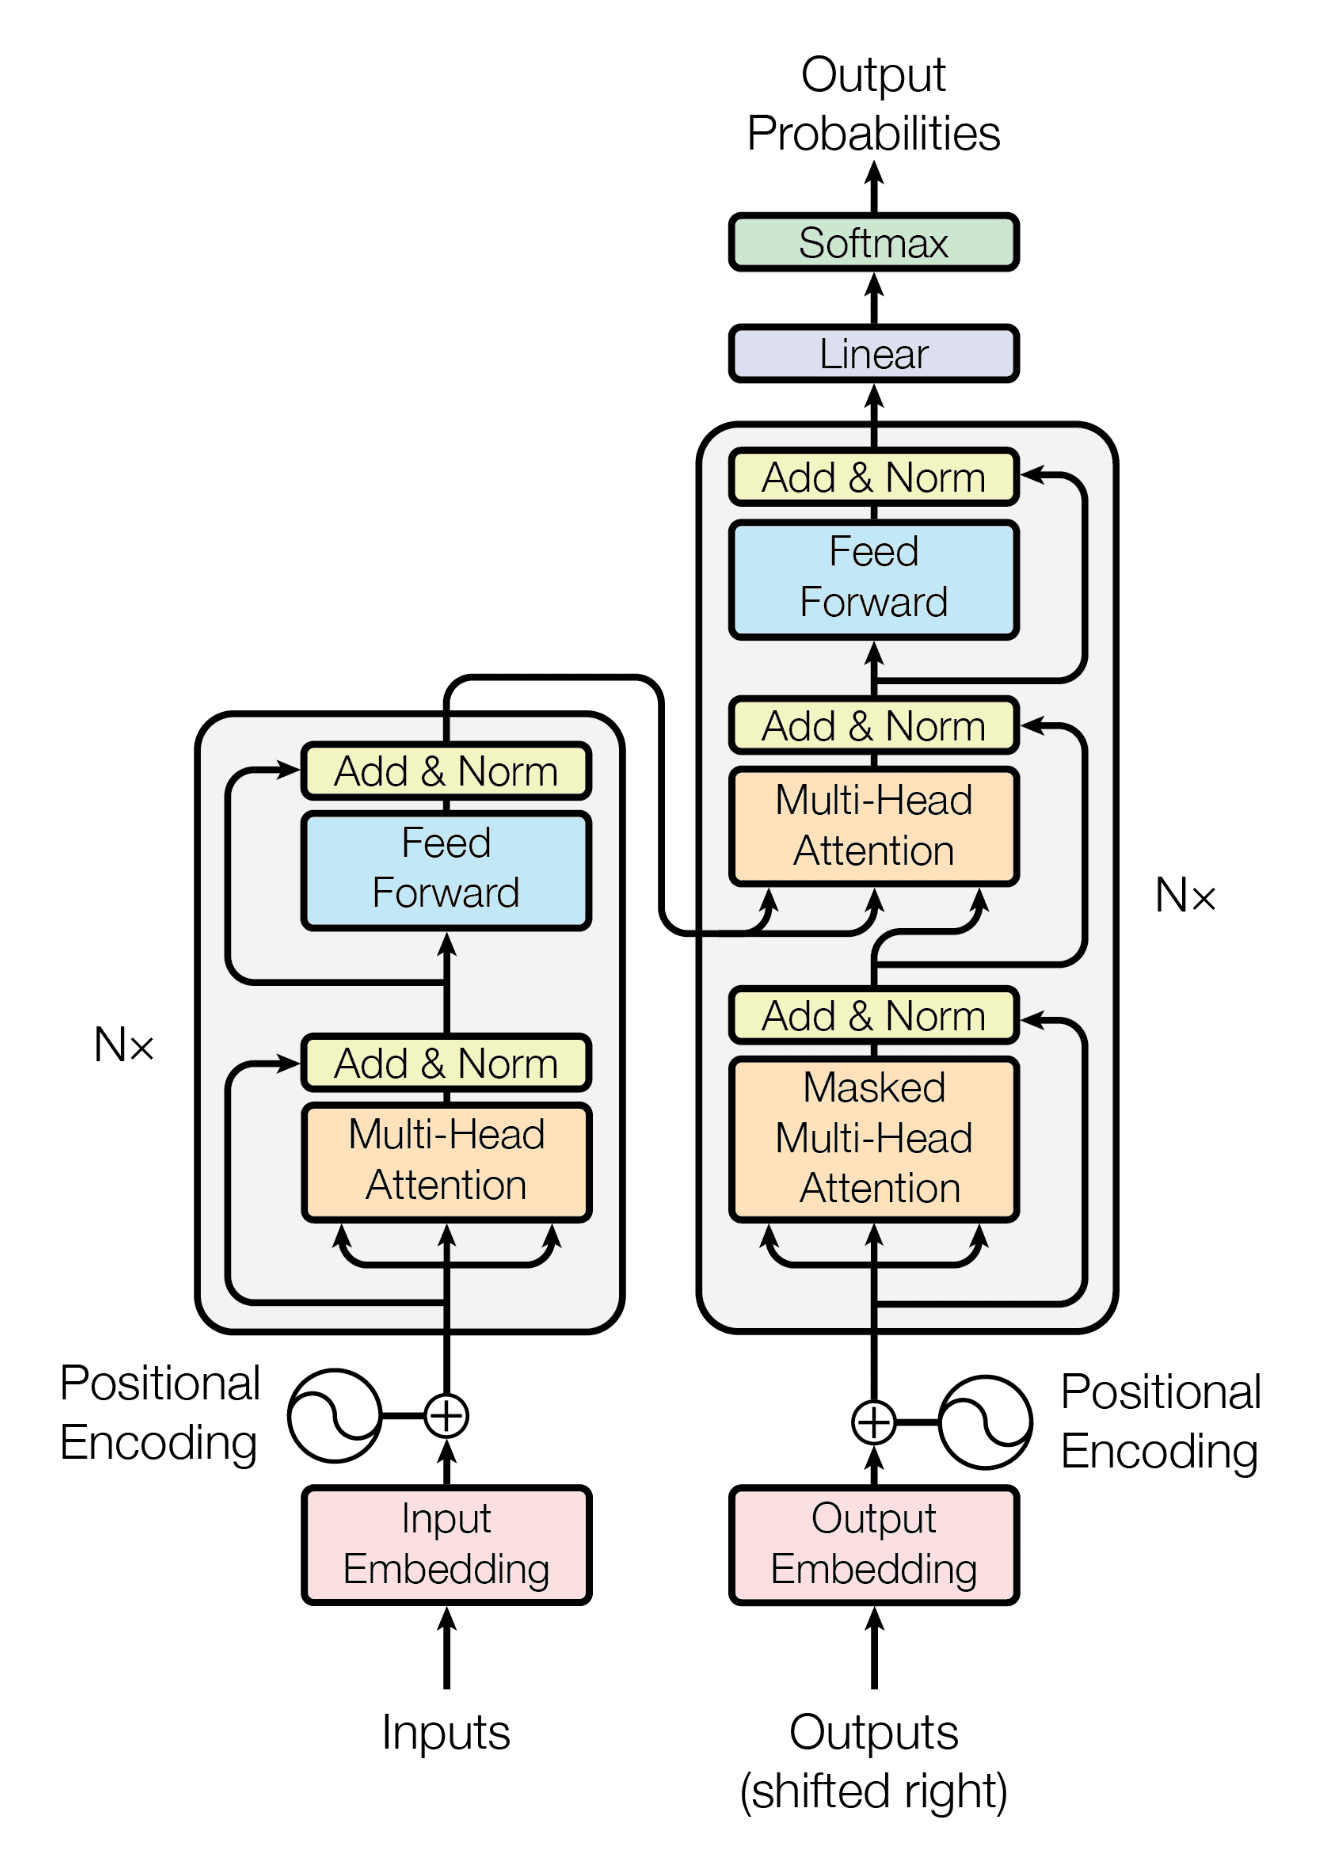
\includegraphics[width=0.7\textwidth]{images/chapter2/transformer.png}
  \caption{\emph{Αρχιτεκτονική Transformer}\\}
  \label{fig:transformer}
\end{figure}
\noindent


Το ζευγάρι \emph{encoder-decoder} εμφανίζεται στη βιβλιογραφία και με τη χρήση αναδρομικών νευρωνικών δικτύων. Ο \emph{encoder} είναι υπεύθυνος για την αντιστοίχηση της διακριτής ακολουθίας συμβόλων εισόδου, $x= [x_1, \cdots, x_n]$, σε μία ακολουθία συνεχών συμβόλων, $z = [z_1, \cdots, z_n]$, ενώ ο \emph{decoder} εφαρμόζει την αντίστροφη διαδικασία για να παράγει την έξοδο, $y = [y_1, \cdots, y_n]$.

\subsection{Επίπεδο προσοχής-Attention}
Προτού τα σύμβολα εισόδου εισέλθουν στο επίπεδο προσοχής, μετατρέπονται σε διανύσματα που ονομάζονται ενσωματώσεις λέξεων\footnote{\url{https://en.wikipedia.org/wiki/Word_embedding}} (\emph{word embeddings}). Στο επίπεδο προσοχής εφαρμόζεται μία συνάρτηση σε κάθε διάνυσμα εισόδου, από την οποία παράγονται τρία νέα διανύσματα για κάθε ένα διάνυσμα $x_i$. Τα τρία διανύσματα αυτά ονομάζονται $query-q$ $key-v$ και $value-v$ και παράγονται από τον πολλαπλασιασμό του διανύσματος $x_i$ με τρεις πίνακες βαρών $W_q$, $W_k$ και $W_v$ αντίστοιχα. Η διαδικασία υπολογισμού του \emph{attention} αποτελεί μία διαδικασία πράξεων πινάκων και εξαιτίας του γεγονότος αυτού πραγματοποιείται πολύ γρήγορα γιατί ο υπολογισμός του μπορεί να γίνει για όλες τις εισόδους $x_i$ ταυτόχρονα.

\subsubsection{\emph{Attention} Σταθμισμένου Εσωτερικού Γινομένου}
Το \emph{attention} σταθμισμένου εσωτερικού γινομένου (\emph{Scaled Dot-Product Attention} υπολογίζεται ως εξής:

\begin{equation}
    \label{eq:attention}
    Attention(Q,K,V) = softmax(\frac{QK^T}{\sqrt{d_k}})V
\end{equation}

όπου στην \autoref{eq:attention}:
\begin{itemize}
    \item $Q$: Πίνακας με τα διανύσματα \emph{query}
    \item $K$: Πίνακας με τα διανύσματα \emph{key}
    \item $d_k$: Η διάσταση των διανυσμάτων \emph{query} και \emph{key}
    \item $V$: Πίνακας μα τα διανύσματα \emph{value}, διάστασης $d_v$
\end{itemize}

\subsection{Attention Πολλαπλής κεφαλής}
Μια παραλλαγή του \emph{scaled dot-product attention} είναι το \emph{attention} πολλαπλής κεφαλής (\emph{multi-head attention}), όπου αντί να εφαρμόζεται μία μονάχα συνάρτηση \emph{attention} εφαρμόζονται πολλαπλές συναρτήσεις με αποτέλεσμα την παραγωγή πολλών διανυσμάτων $q$, $k$, $v$ για κάθε μία από τις εισόδους $x_i$. Αυτή η παραλλαγή βοηθάει ώστε το μοντέλο να μπορεί να επικεντρωθεί σε πολλά τμήματα τις ακολουθίας εισόδου ταυτόχρονα. Η μαθηματική έκφραση του \emph{multi-head attention} φάινεται στην \autoref{eq:multi-head}. Η μάσκα που εφαρμόζεται στο επίπεδο του \emph{decoder} εφαρμόζεται έτσι ώστε οι προβλέψεις για τη θέση $i$ να εξαρτώνται μόνο από τις γνωστές εξόδους που προηγήθηκαν της $i$ και όχι από "μελλοντικές".

\begin{equation} \label{eq:multi-head}
\begin{split}
    MultiHead(Q,K,V) = Concat(head_1, \cdots, head_h)W^O \\
    head_i= Attention(QW_i^Q, KW_i^K,VW_i^V)
\end{split}
\end{equation}

όπου:
\begin{itemize}
    \item $d_{model}$: Η διάσταση των διανυσμάτων εξόδου του μοντέλου
    \item $W^Q \in \mathbb{R}^{d_{model} \times hd_k} $
    \item $W^K \in \mathbb{R}^{d_{model}\times  hd_k} $
    \item $W^V \in \mathbb{R}^{d_{model} \times  hd_v} $
    \item $W^O \in \mathbb{R}^{d_{model}\times  hd_k} $
\end{itemize}

Η έξοδος του επιπέδου \emph{multi-head attention}, αφού πρώτα αθροιστεί και κανονικοποιηθεί, εισέρχεται σε ένα απλό \emph{feed-forward} πλήρως συνδεδεμένο NN το οποίο χρησιμοποιεί συνάρτηση ενεργοποίησης \emph{ReLU}\footnote{\url{https://en.wikipedia.org/wiki/Rectifier_(neural_networks)}}.